\documentclass[12pt,fleqn]{article}
\setlength{\parindent}{0pt}
\usepackage{graphicx}
\usepackage{cancel}
\usepackage{listings}
\usepackage[latin5]{inputenc}
\usepackage{color}
\setlength{\parskip}{8pt}
\setlength{\parsep}{0pt}
\setlength{\headsep}{0pt}
\setlength{\topskip}{0pt}
\setlength{\topmargin}{0pt}
\setlength{\topsep}{0pt}
\setlength{\partopsep}{0pt}
\setlength{\mathindent}{0cm}
\usepackage{latexsym}
\usepackage{amsfonts}
\usepackage{mathrsfs}
\usepackage{showkeys}
\renewcommand*\showkeyslabelformat[1]{(#1)}

\begin{document}
Ders 24

Green'in Teorisinin iki seklini gormustuk

\[ \oint_C \vec{F} \cdot \vec{T} ds = \int \int_R curl \ \vec{F} \ dA \]

\[ \oint_C \vec{F} \cdot \vec{n} \ ds = \int \int_R div \ \vec{F} \ dA \]


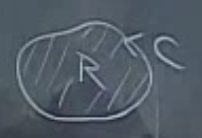
\includegraphics[height=2cm]{24_1.png}

Bu esitliklerin sol tarafi icin $\vec{F}$'in sadece $C$ uzerinde tanimli
olmasi yeterlidir. Fakat esitliklerin anlamli olmasi icin, yani sag
tarafinin da dogru olmasi icin $\vec{F}$'in $R$ icindeki her noktada tanimli
olmasi gerekir. Eger $R$ icinde tanimli olmayan tek bir nokta bile varsa, o
zaman ustteki esitlikleri kullanamayiz.

Ornek 

\[ \vec{F} = \frac{ -y\hat{i} + x\hat{j}}{x^2+y^2} \]

Ustteki $\vec{F}$ orijinde tanimli degildir, diger her yerde , $curl \
\vec{F} = 0$. 
Iki olasiliga bakalim, diyelim ki ``sekilsel'' olarak benzer alanlar orijini
iceren, bir de icermeyen sekillerde verilmis

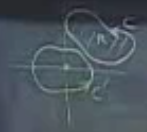
\includegraphics[height=3cm]{24_2.png}

 















\end{document}
